\documentclass[a4paper,10pt]{tufte-book}

\usepackage{listings}
\usepackage{color}
\usepackage[usenames,dvipsnames]{xcolor}
\usepackage{moreverb}
\usepackage{graphicx}
\usepackage{subfigure}
\usepackage{float}
\usepackage{booktabs}
\usepackage{hyperref}
\usepackage[toc,page]{appendix}

\usepackage{titlesec}
\usepackage[framemethod=TikZ]{mdframed}
\usepackage{tikz}\usetikzlibrary{shapes.misc}
\newcommand\qnhead{\vspace{0.25cm}%
\tikz[baseline,trim left=3.1cm, trim right=3cm] {
        \fill [black!12] (2.5cm,-1ex) rectangle (\textwidth+3.3cm,2.5ex);
        \node [
            anchor= base east,
            rectangle,
            minimum height=3.5ex] at (3cm,0ex) {
    \thesection
};
}\vspace{0.25cm}}
\renewcommand{\thesection}{}

\title{SparQLed\\
{\normalsize --- Assisted SPARQL Editor through RDF Graph Analytics}}

\begin{document}

\maketitle

\newthought{SparQLed is an interactive SPARQL editor} that helps users in formulating complex SPARQL queries across multiple heterogeneous data sources. Whether or not the structure and vocabulary of data sources are known, users can easily formulate queries through various kinds of context-aware element recommendations.

This document presents the steps to setup the editor:
\begin{enumerate}
\item Compute the Data Graph Summary;
\item Configure the webapp;
\item Launch the SparQLed webapp.
\end{enumerate}

\qnhead{The Data Graph Summary}

SparQLed makes use of the entire query structure and of the Data Graph Summary~\cite{campinas:dexa:2012} (DGS) in order to present to the user possible query elements.

The DGS has to be calculated beforehand and contains a statistical description of the underlying data. The DGS is depicted in Figure~\ref{fig:dgs-model}, where the bottom layer, i.e., the original RDF data, is condensed into the graph represented on the middle layer. For example, the resources of type Person are represented with the single resource labelled Person, where a cardinality indicates how many resources were aggregated.

\begin{marginfigure}
\centering
    \resizebox{\linewidth}{!}{
    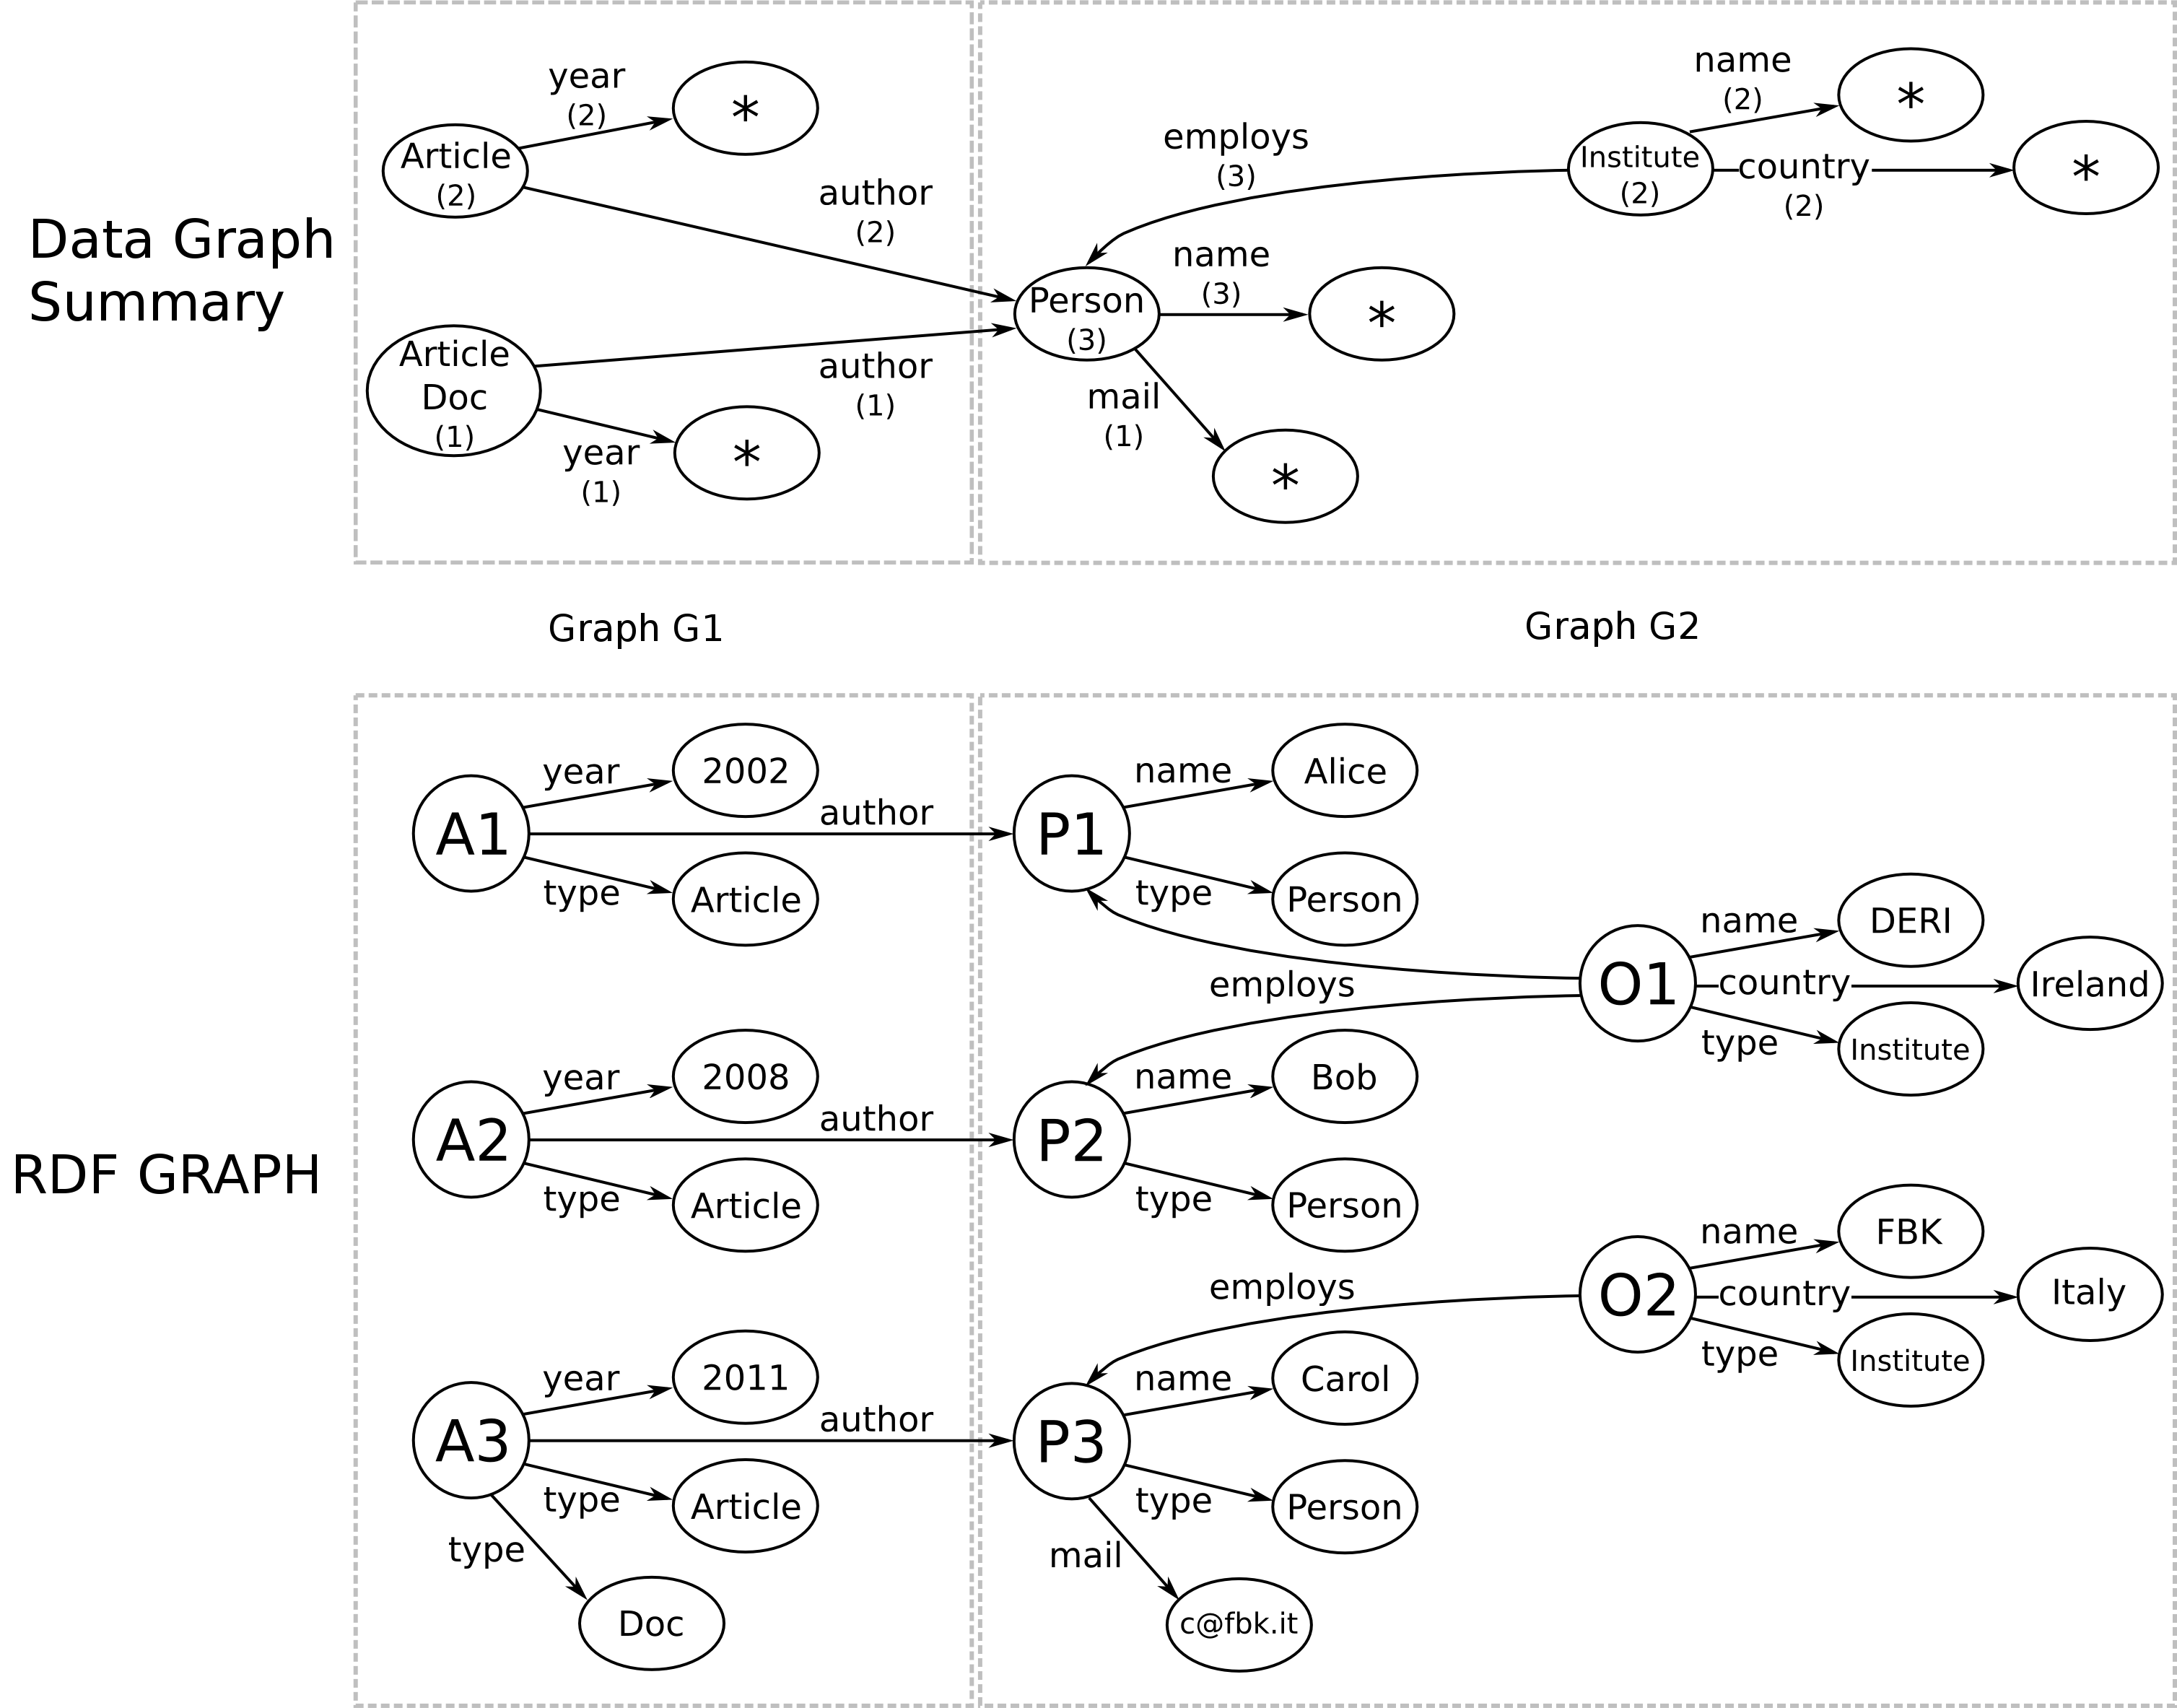
\includegraphics[scale=1]{figures/model.png}}
    \caption{Layers of the Data Graph Summary Model}
    \label{fig:dgs-model}
\end{marginfigure}

The DGS is represented again in RDF using the \emph{Dataset Analytics Vocabulary\footnote{\url{http://vocab.sindice.net/analytics}}} ontology. Usually considerably smaller than the original RDF Graph, it is accessed by the Sparqled via SPARQL. For querying and exploring the DGS outside of SparQLed see the Appendix.


\qnhead{0. Getting Started}

The following needs to be installed:
\begin{itemize}
\item Tomcat6\footnote{\textcolor{blue}{on Ubuntu, sudo apt-get install tomcat6}} or Tomcat7;
\item Maven3;
\item Java 1.6.0\_*;
\item a SPARQL endpoint with SPARQL1.1 support.
\end{itemize}

The following command creates the file \emph{sparql-summary-assembly.jar} in the directory \emph{target/}. It is used to compute the Data Graph Summary and other operations on a SPARQL endpoint:

\bigskip
\begin{raggedleft}
\framebox[\linewidth][l]{
    \parbox[r]{\linewidth}{\texttt{
        \$ mvn -{}-projects sparql-summary package assembly:assembly -{}-also-make
    }}
}
\end{raggedleft}

A detailed explanation of the \texttt{sparql-summary-assembly.jar} command line interface is found in the README file, in the \texttt{sparql- summary} module.


\qnhead{1. Computing the Data Graph Summary}

The DGS implementation bundled with this documentation is based on SPARQL, and computes the summary over a single dataset. A high performance, hadoop-based, DGS implementation is also available, and allows to compute a summary across datasets. Therefore, links between datasets can also be recommended. However, this version is not shipped with this package. Please inquire\footnote{\url{http://groups.google.com/group/sindice-dev}}.

The following command will create the DGS over the given dataset which lies in a SPARQL endpoint located at \url{http://url/to/sparql/endpoint/}. The output is a gzip compressed NTriple file \texttt{/path/to/\mbox{$<\!data\!>$}-summary.nt.gz}. It is strongly advised to give enough memory to prevent OOME, e.g., \texttt{-Xmx2048m}.

\bigskip
\begin{raggedleft}
\framebox[\linewidth][l]{
    \parbox[r]{\linewidth}{\texttt{
        \$ java -cp target/sparql-summary-assembly.jar org.sindice.summary.Pipeline -{}-type HTTP -{}-repository \url{http://url/to/sparql/endpoint/} -{}-outputfile /path/to/\mbox{$<\!data\!>$}-summary.nt.gz
    }}
}\marginnote[-0.8cm]{\textcolor{blue}{You can constrain the processing to a single named graph using the option \texttt{-{}-domain}.}}
\end{raggedleft}
\hfill

A SPARQL endpoint must then be loaded with the computed DGS NTriples, under the named graph \url{http://sindice.com/analytics}.


\qnhead{2. Configuring the Webapp}

In this section and the next, we use by default tomcat6. If you are to use tomcat7, replace all occurrences of tomcat6 by tomcat7.

In order to properly configure the application, we need to stop tomcat:

\bigskip
\begin{raggedleft}
\framebox[\linewidth][l]{
    \texttt{
        \$ sudo service tomcat6 stop
    }
}
\end{raggedleft}

\subsection{Edit Tomcat Properties}

The application needs to set a pre-defined folder, where it can read configuration settings and also writes log output into a file. That folder is set using the Tomcat property \texttt{sindice.home} to the value \texttt{/path/to/sindice/home}.

As a super-user, edit the file \texttt{/etc/default/tomcat6} and update the \texttt{JAVA\_OPTS} variable:

\bigskip
\begin{raggedleft}
\framebox[\linewidth][l]{
    \texttt{
        JAVA\_OPTS="-Dsindice.home=/path/to/sindice/home"
    }
}
\end{raggedleft}
\hfill

Set tomcat6 permissions on that folder, so that the deployed webapp can write in that folder:

\bigskip
\begin{raggedleft}
\framebox[\linewidth][l]{
    \texttt{
        \$ sudo chown -R tomcat6:tomcat6 /path/to/sindice/home
    }
}
\end{raggedleft}

\subsection{Create the Webapp .war File}

Edit the default XML config file of SparQLed:

\bigskip
\begin{raggedleft}
\framebox[\linewidth][l]{
    {\small \texttt{
        recommendation-servlet/src/main/resources/default-config.xml
    }}
}
\end{raggedleft}

Set\marginnote{\textcolor{blue}{{\bfseries recommender} and {\bfseries proxy} tags}} the URL to the endpoints loaded with the original RDF Graph and the DGS. The endpoint with the RDF Graph is set under the \texttt{proxy} tag, the one with the DGS graph is set under the \texttt{recommender} tag.

We assume here that both graphs are loaded into the same, \texttt{HTTP} endpoint:

\bigskip
\begin{raggedleft}
\framebox[\linewidth][l]{
    \parbox[r]{\linewidth}{\texttt{
        <backendArgs>http://path/to/sparql/endpoint</backendArgs>
    }}
}
\end{raggedleft}
\hfill

The \texttt{sparqled.war} file is created using the following command, and is located in the directory \texttt{recommendation-servlet/target/}:

\bigskip
\begin{raggedleft}
\framebox[\linewidth][l]{
    \parbox[r]{\linewidth}{\texttt{
        \$ mvn -{}-projects recommendation-servlet -{}-also-make package
    }}
}
\end{raggedleft}

\qnhead{3. Launching the SparQLed Webapp}
\label{sec:sparqled}

With the SPARQL endpoint ready and the configuration files correctly setup, we are now ready to launch the webapp!

\subsection{Clean Previously Installed Webapp}

Remove a previously deployed SparQLed webapp, in order to avoid unexpected issues:

\bigskip
\begin{raggedleft}
\framebox[\linewidth][l]{
    \parbox[r]{\linewidth}{\texttt{
        \$ rm -rf /path/to/sindice/home/sparqled\\\hspace{0.02cm}
        \$ rm -rf \$CATALINA\_BASE/webapps/sparqled*
    }}
}\marginnote[-0.2cm]{\textcolor{blue}{On Ubuntu, \$CATALINA\_BASE=/var/lib/tomcat6/}}
\end{raggedleft}

\subsection{Run Tomcat}

Copy the \texttt{sparqled.war} file to the tomcat base directory and start tomcat:

\bigskip
\begin{raggedleft}
\framebox[\linewidth][l]{
    \parbox[r]{\linewidth}{\texttt{
        \$ sudo cp recommendation-servlet/target/sparqled.war \$CATALINA\_BASE/webapps/\\\hspace{0.002cm}
        \$ sudo service tomcat6 start
    }}
}
\end{raggedleft}


\qnhead{Using SparQLed}

If no problem, the SparQLed (Figure~\ref{fig:sparqled}) webapp is available at:

\bigskip
\begin{raggedleft}
\framebox[\linewidth][l]{
    \texttt{
        \url{http://localhost:8080/sparqled/}
    }
}
\end{raggedleft}

\begin{marginfigure}
    \resizebox{\linewidth}{!}{
    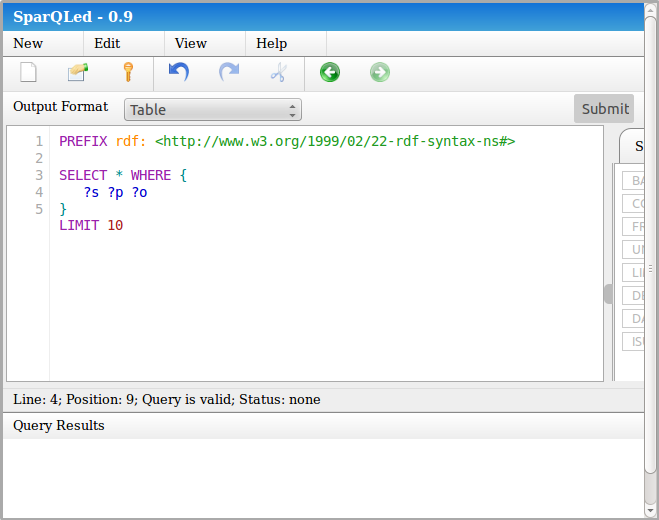
\includegraphics[scale=1]{figures/window.png}}
    \caption{The SparQLed editor}
    \label{fig:sparqled}
\end{marginfigure}
 
In case the webapp does not work properly, please have a look at the logs:

\bigskip
\begin{raggedleft}
\framebox[\linewidth][l]{
    \parbox[r]{\linewidth}{\texttt{
        \$ tail -f \$CATALINA\_BASE/logs/catalina.out\\\hspace{0.002cm}
        \$ tail -f /path/to/sindice/home/log/sparqled/sparqled.log
    }}
}
\end{raggedleft}

The SparQLed\footnote{\textcolor{blue}{A live version and a screencast are available at \url{http://hcls.sindicetech.com/sparql-editor/}}} editor gives you four types of recommendations, i.e., class, predicate, relationship between variables and named graphs.

In order to get recommendations you have to hit \texttt{Ctrl + Space} at the desired position in the query. The recommendations generated by the editor will be provided in the form of a drop down list. The user can then select one entry from the drop down box that matches his criteria. Keyword (resp., prefix) search is also possible by typing a word (resp., prefix), followed by \texttt{Ctrl + Space}.



\qnhead{KNOWN ISSUES}

The editor use the SPARQL1.0 grammar. Therefore, there is no syntax highlighting nor syntax recommendations\footnote{\textcolor{blue}{not to be confused with the structural recommendations the SparQLed provides}} for SPARQL1.1 keywords. However, it is still possible to submit a 1.1 query to the endpoint. This issue will be resolved in the near future.

\qnhead{ACKNOWLEDGEMENT}

This software is based upon works supported by the European FP7 project LOD2 (257943).

\qnhead{CONTACT}

If you have any questions or issues, please contact us at \url{http://groups.google.com/group/sindice-dev}.

\bibliography{sparqled-doc}
\bibliographystyle{plainnat}

\appendix
\clearpage
\chapter{Appendix}

\section{A. How to Query the Data Graph Summary ?}

The Data Graph Summary is modeled using the \emph{Dataset Analytics Vocabulary\footnote{\url{http://vocab.sindice.net/analytics}}} ontology. Below are some examples on how to use the Data Graph Summary.

\begin{itemize}
\item The following query returns the properties used with the class \url{http://schema.org/Person} in the dataset \texttt{bbc.co.uk}:

\lstset{language=SQL,basicstyle=\footnotesize}
\begin{lstlisting}
PREFIX an: <http://vocab.sindice.net/analytics>
PREFIX any23: <http://vocab.sindice.net/>
PREFIX d: <http://sindice.com/dataspace/default/domain/>

SELECT DISTINCT ?Predicate
FROM <http://sindice.com/analytics>
WHERE {
    ?node an:label ?l .
    ?l an:label <http://schema.org/Person> .
    
    ?edge an:source ?node ;
          an:label ?Predicate ;
          an:publishedIn d:bbc.co.uk .
}
LIMIT 20
\end{lstlisting}


\item The following query returns the most used classes in a dataset:

\lstset{language=SQL,basicstyle=\footnotesize}
\begin{lstlisting}
PREFIX an: <http://vocab.sindice.net/analytics>
PREFIX any23: <http://vocab.sindice.net/>

SELECT ?Dataset ?Class (SUM(?card) AS ?Cardinality)
FROM <http://sindice.com/analytics>
WHERE {
    ?node any23:dataset_uri ?Dataset ;
          an:cardinality ?card ;
          an:label ?l .
    ?l an:label ?Class .
}
GROUP BY ?Dataset ?Label
ORDER BY DESC(?Cardinality)
LIMIT 20
\end{lstlisting}
\end{itemize}

\section{B. How to setup SparQLed from scratch ?}

In this Section, we assume that you have no SPARQL endpoint and no RDF data available. We explain you how to setup a SparQLed instance from scratch.

\subsection{Example Datasets}

One may download one of the following datasets:
\begin{itemize}
    \item the European Nature Information System\footnote{\textcolor{blue}{\url{http://thedatahub.org/dataset/eunis}}} dataset (large, long setup):

    \begin{raggedleft}
    \framebox[\linewidth][l]{
        \parbox[r]{\linewidth}{\texttt{
            \$ wget http://eunis.eea.europa.eu/rdf/\{sites,habitats,\\\hspace{0.5cm}species,taxonomies\}.rdf.gz -{}-directory-prefix eunis
        }}
    }
    \end{raggedleft}

    \item the New York Times - Linked Open Data\footnote{\textcolor{blue}{\url{http://thedatahub.org/dataset/nytimes-linked-open-data}}} dataset (small, fast setup):

    \begin{raggedleft}
    \framebox[\linewidth][l]{
        \parbox[r]{\linewidth}{{\small\texttt{
            \$ wget http://data.nytimes.com/\{locations,organizations,\\\hspace{0.5cm}people,descriptors\}.rdf -{}-directory-prefix nytimes
        }}}
    }
    \end{raggedleft}
\end{itemize}

We need to load the downloaded RDF data into a SPARQL endpoint.
We create here a Sesame Native\footnote{\textcolor{blue}{\url{http://www.openrdf.org/doc/sesame2/users/ch07.html}}} endpoint:

\bigskip
\begin{raggedleft}
\framebox[\linewidth][l]{
    \parbox[r]{\linewidth}{\texttt{
        \$ java -cp target/sparql-summary-assembly.jar org.sindice.summary.Pipeline -{}-feed -{}-type NATIVE -{}-repository /path/to/\mbox{$<\!data\!>$}-native -{}-add /path/to/\mbox{$<\!data\!>$} -{}-addformat=RDF/XML
    }}
}
\end{raggedleft}
\hfill

The format of the ingested RDF data is in NTriples by default. A different format can be given through the option \texttt{\mbox{-{}-addformat}}.

\subsection{Compute the Data Graph Summary}

To compute the DGS over the downloaded data, we will execute SPARQL queries against the previous Native repository. This creates the file \texttt{/path/to/\mbox{$<\!data\!>$}-summary.nt.gz} containing the summary in the NTriple format.

\bigskip
\begin{raggedleft}
\framebox[\linewidth][l]{
    \parbox[r]{\linewidth}{\texttt{
        \$ java -cp target/sparql-summary-assembly.jar org.sindice.summary.Pipeline -{}-type NATIVE -{}-repository /path/to/\mbox{$<\!data\!>$}-native -{}-outputfile /path/to/\mbox{$<\!data\!>$}-summary.nt.gz
    }}
}
\end{raggedleft}
\hfill

We load the DGS triples into a new Sesame Native repository \texttt{/path/to/\mbox{$<\!data\!>$}-summary-native} under the named graph \url{http://sindice.com/analytics}. The reason to create a new repository is that Sesame locks the Native repository when in use, preventing another connection to be made.

\bigskip
\begin{raggedleft}
\framebox[\linewidth][l]{
    \parbox[r]{\linewidth}{\texttt{
        \$ java -cp target/sparql-summary-assembly.jar org.sindice.summary.Pipeline -{}-feed -{}-type NATIVE -{}-repository /path/to/\mbox{$<\!data\!>$}-summary-native -{}-domain http://sindice.com/analytics -{}-add /path/to/\mbox{$<\!data\!>$}-summary.nt.gz
    }}
}
\end{raggedleft}
\hfill

\subsection{Configure the Webapp}

Since we are now using a Native repository, the SparQLed configuration file needs to be updated:
\begin{itemize}
\item Edit the SparQLed XML configuration file:

\bigskip
\begin{raggedleft}
\framebox[\linewidth][l]{
    {\small \texttt{
        recommendation-servlet/src/main/resources/default-config.xml
    }}
}
\end{raggedleft}

\item Edit both endpoints, i.e., for the original RDF Graph and for the DGS, to point to the Native repositories:

\bigskip
\begin{raggedleft}
\framebox[\linewidth][l]{
    \parbox[r]{\linewidth}{\texttt{
        <backend>NATIVE</backend>\\\hspace{0.02cm}
        <backendArgs>/path/to/\mbox{$<\!data\!>$}-native</backendArgs>
    }}
}\marginnote{\textcolor{blue}{{\bfseries proxy} tag}}
\end{raggedleft}

\bigskip
\begin{raggedleft}
\framebox[\linewidth][l]{
    \parbox[r]{\linewidth}{{\small\texttt{
        <backend>NATIVE</backend>\\\hspace{0.02cm}
        <backendArgs>/path/to/\mbox{$<\!data\!>$}-summary-native</backendArgs>
    }}}
}\marginnote{\textcolor{blue}{{\bfseries recommender} tag}}
\end{raggedleft}
\end{itemize}

\subsection{Launching the SparQLed Webapp}

Before following the steps detailed in the Section~3, you have to grant tomcat6 (or, tomcat7) the ownership to the native repositories:

\bigskip
\begin{raggedleft}
\framebox[\linewidth][l]{
    \parbox[r]{\linewidth}{{\small\texttt{
        \$ sudo chown -R tomcat6:tomcat6 /path/to/\mbox{$<\!data\!>$}-native\\\hspace{0.02cm}
        \$ sudo chown -R tomcat6:tomcat6 /path/to/\mbox{$<\!data\!>$}-summary-native
    }}}
}
\end{raggedleft}



\end{document}
